	\pagenumbering{roman}
	
	\chapter{Anhang}
	
	\section{Code der Algorithmen}
	
	\subsection{Dijkstra}
	
	\begin{lstlisting}
(* Implementation of the Dijkstra algorithm as a possible heuristic for the A* algorithm and for static pathfinding.*)

// set return to false
#FC_buildHeuristicList := false;

// initialize PrioQueue
"FC_buildHpq"( targetNodeID:=#nodeID, priorityQueue:=#priorityQueue);


// while still nodes in Prioqueue
#heuristicCounter := 0;
WHILE #priorityQueue.numberOfNodes > 0 DO

	// get node with smallest distance
	"FC_hpqPop"(hpq := #priorityQueue, poppedNode => #tempCurrentNode);
	#tempAdjIndex := #tempCurrentNode.nodeID;
	
	//check all connected nodes
	FOR #adjCounter := 0 TO #adjMatrix.numberOfNodes - 1 DO
	
		// temp Adj Index as second index, adj counter as first, to get edges leading to target and not from the target. 
		#tempDistance := #adjMatrix.adjacencyMatrix[#adjCounter, #tempAdjIndex];
		IF #tempDistance <> 0 THEN
		
		// relax edges
		IF #tempCurrentNode.distanceToStartNode = "DIST_INFINITE" THEN
		#tempNewDistance := "DIST_INFINITE";
		ELSE
		#tempNewDistance := #tempCurrentNode.distanceToStartNode + #tempDistance;
		END_IF;
		
		#tempUpdateSuccess := "FC_updateNodeHpq"(hpq:= #priorityQueue,NodeID:= #adjCounter,potNewDistance:= (#tempNewDistance),potParent:= #tempCurrentNode.nodeID);
		"FC_hpqSort"(prioQueue := #priorityQueue);
		
		END_IF;
	END_FOR;
	
	//add done nodes to heuristics list
	#heuristicList.heuristicList[#heuristicCounter] := #tempCurrentNode;
	#heuristicList.nodeIDList[#heuristicCounter] := #tempCurrentNode.nodeID;
	#heuristicList.numberOfNodes := #heuristicList.numberOfNodes + 1;
	#heuristicCounter := #heuristicCounter + 1;
END_WHILE;

#FC_buildHeuristicList := true;
	\end{lstlisting}

	\subsection{A*}
	
	\begin{lstlisting}
// set default conditions
IF #start = true AND #statDone = true THEN
	"DB_Debug".countPF := "DB_Debug".countPF + 1;
	#statPathfindingNodeList.numberOfNodes := 0;
	
	// clear PPQ and closed list first
	WHILE #ppqOpenlist.numberOfNodes > 0 DO
	"FC_ppqPop"(poppedNode => #tempPpqPoppedNode,
	ppq := #ppqOpenlist);
	END_WHILE;
	
	FOR #counter := 0 TO #statAlreadyVisited.numberOfNodes DO
	#statAlreadyVisited.closedList[#counter] := -1;
	END_FOR;
	#statAlreadyVisited.numberOfNodes := 0;
	
	//create start node
	#tempPpqStartNode.nodeID := #sourceID;
	#tempPpqStartNode.parentID := #sourceID;
	#tempPpqStartNode.currRouteDistance := 0;
	#tempPpqStartNode.expectedRouteDistance := "FC_getHeuristicValue"(heuristicList := #targetTable.heuristicTable[#statHeuristicListIndex].targetHeuristic,
	queryID := #sourceID);
	
	// add start node to openlist
	"FC_ppqInsert"(newNode := #tempPpqStartNode,
	ppq := #ppqOpenlist);
	// select Heuristicstable entry corresponding to target
	"FC_getHeuristicListIndex"(heuristicTable := #targetTable,
	tableIndex => #statHeuristicListIndex,
	targetSearchID := #targetID);
	
	//set start and done to false
	#start := false;
	#statDone := false;
END_IF;

//if right heuristic list selected from heuristic table for current target
IF #targetID = #targetTable.heuristicTable[#statHeuristicListIndex].targetID THEN

	//while still items in the openlist
	IF #ppqOpenlist.numberOfNodes > 0  AND #statDone = false THEN 
	
		//extract node with shortest distance
		"FC_ppqPop"(poppedNode => #tempPpqPoppedNode,
		ppq := #ppqOpenlist);
		
		#tempCurrNodeID := #tempPpqPoppedNode.nodeID;
		
		//add node to closed list, as to not visit it again
		"FC_addToClosedList"(closedList := #statAlreadyVisited,
		nodeId := #tempCurrNodeID);
		
		#tempCurrRouteDist := #tempPpqPoppedNode.currRouteDistance;
		
		//if target was reached, break the loop
		IF #tempCurrNodeID = #targetID THEN
			#statPathfindingNodeList.nodeList[#statPathfindingNodeList.numberOfNodes] := #tempPpqPoppedNode;
			#statPathfindingNodeList.numberOfNodes := #statPathfindingNodeList.numberOfNodes + 1;
			#statDone := true;
		
		
		ELSE
		
			//search all nodes for connections
			FOR #counter := 0 TO "MAX_INDEX_NODES_PF" DO
			
				IF #vacancyMatrix.vacancyMatrix[#tempCurrNodeID, #counter] THEN
					#tempDistToConnectedNode := #adjMatrix.adjacencyMatrix[#tempCurrNodeID, #counter];
					
					// if node is connected
					IF #tempDistToConnectedNode <> 0 THEN
					
						// check if next next node is blocked because of vehicle, if yes make more costly
						IF #tempCurrNodeID = #sourceID AND #counter = #blockedNextID THEN
							#tempDistToConnectedNode := #tempDistToConnectedNode + #ADDITIONAL_BLOCKED_ADJUSTMENT;
						END_IF;
						
						"FC_ppqContains"(ppq := #ppqOpenlist,
						searchID := #counter,
						searchIndex => #tempContainsIndex);
						
						#tempHeurValue := "FC_getHeuristicValue"(heuristicList := #targetTable.heuristicTable[#statHeuristicListIndex].targetHeuristic,
						queryID := #counter);
						
						//if node is not yet in openlist, check if already closed. If not, add to openlist
						#tempAlreadyClosed := "FC_CheckIfInClosedList"(closedList := #statAlreadyVisited,
						nodeID := #counter);
						IF #tempContainsIndex = -1 AND NOT #tempAlreadyClosed THEN
							#tempPpqInsertNode.nodeID := #counter;
							#tempPpqInsertNode.parentID := #tempCurrNodeID;
							#tempPpqInsertNode.currRouteDistance := #tempCurrRouteDist + #tempDistToConnectedNode;
							#tempPpqInsertNode.expectedRouteDistance := #tempPpqInsertNode.currRouteDistance + #tempHeurValue;
							"FC_ppqInsert"(newNode := #tempPpqInsertNode,
							ppq := #ppqOpenlist);
						
						// else update node if necessary
						ELSE
							"FC_updateNodePpq"(NodeID := #counter,
							potNewDistance := #tempCurrRouteDist + #tempHeurValue + #tempDistToConnectedNode,
							potParent := #tempCurrNodeID,
							ppq := #ppqOpenlist);
						END_IF;
					END_IF;
				END_IF;
			END_FOR;
			
			#statPathfindingNodeList.nodeList[#statPathfindingNodeList.numberOfNodes] := #tempPpqPoppedNode;
			#statPathfindingNodeList.numberOfNodes := #statPathfindingNodeList.numberOfNodes + 1;
		END_IF;
	END_IF;
	
	// end when no more nodes in pq
	IF #ppqOpenlist.numberOfNodes = 0 THEN
		#statDone := true;
	END_IF;
	
	// write static pathfinding list to output when done turns true
	"R_TRIG_DB_7"(CLK := #statDone,
	Q => #tempEdgeDone);
	IF #tempEdgeDone THEN
		#pathfindingNodeList := #statPathfindingNodeList;
	END_IF;
	#done := #statDone;
END_IF;
	\end{lstlisting}
	
\section{Steuerungen}
	
	\subsection{Vergleich der verwendeten Steuerungen.}
	
	\begin{table}[H]
		\centering
		\begin{longtable}{| c || c | c | c |}
			\hline
			CPU & 1214C & 1215C & ET200SP(1510SP)\\ \hline
			Arbeitsspeicher & 100kB & 125kB & Prog: 100kB, Dat: 750kB\\ \hline
			Ladespeicher & \multicolumn{2}{c|}{1MB+SD-Card} & SD-Karte(max 32GB)\\ \hline
			Max.Bausteingröße & 64kB & 64kb & DB: 750kb, Rest: 100kB\\ \hline
			Max.Schachtelungstiefe & 16 & 16 & 24 \\ \hline
			Befehlsausführgeschw. & 1780ns & 1780ns & 461ns\\ \hline
		\end{longtable}
		\vspace{0.2cm}
		\caption{Vergleich der für die Wegfindung relevanten Hardwareeigenschaften der verwendeten Steuerungen \cite{S7-1200}\cite{ET200SP}.}
	\end{table}	
		

	\subsection{Speicherverbrauch}
	
	\begin{figure}[H]
		\centering
		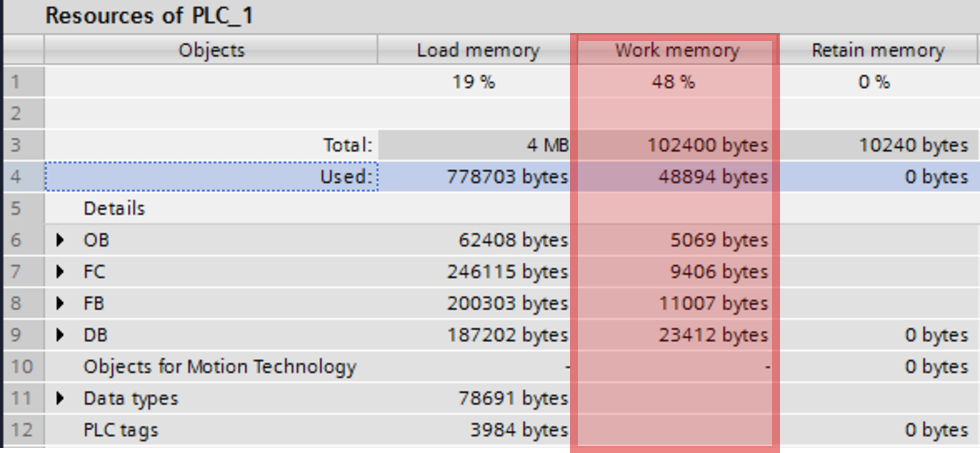
\includegraphics[scale=0.9]{/Bilder/SpeicherverbrauchPDF}
		\vspace{0.2cm}
		\caption{Speicherverbrauch des gesammten Anwenderprogramms inkl. Fahrsteuerung und Kommunikation. 48\% Arbeitsspeicherbelegung auf der kleinsten 1214C-Steuerung.}
	\end{figure}

\section{Aufbau der Datentypen}

	\begin{figure}[h]
		\centering
		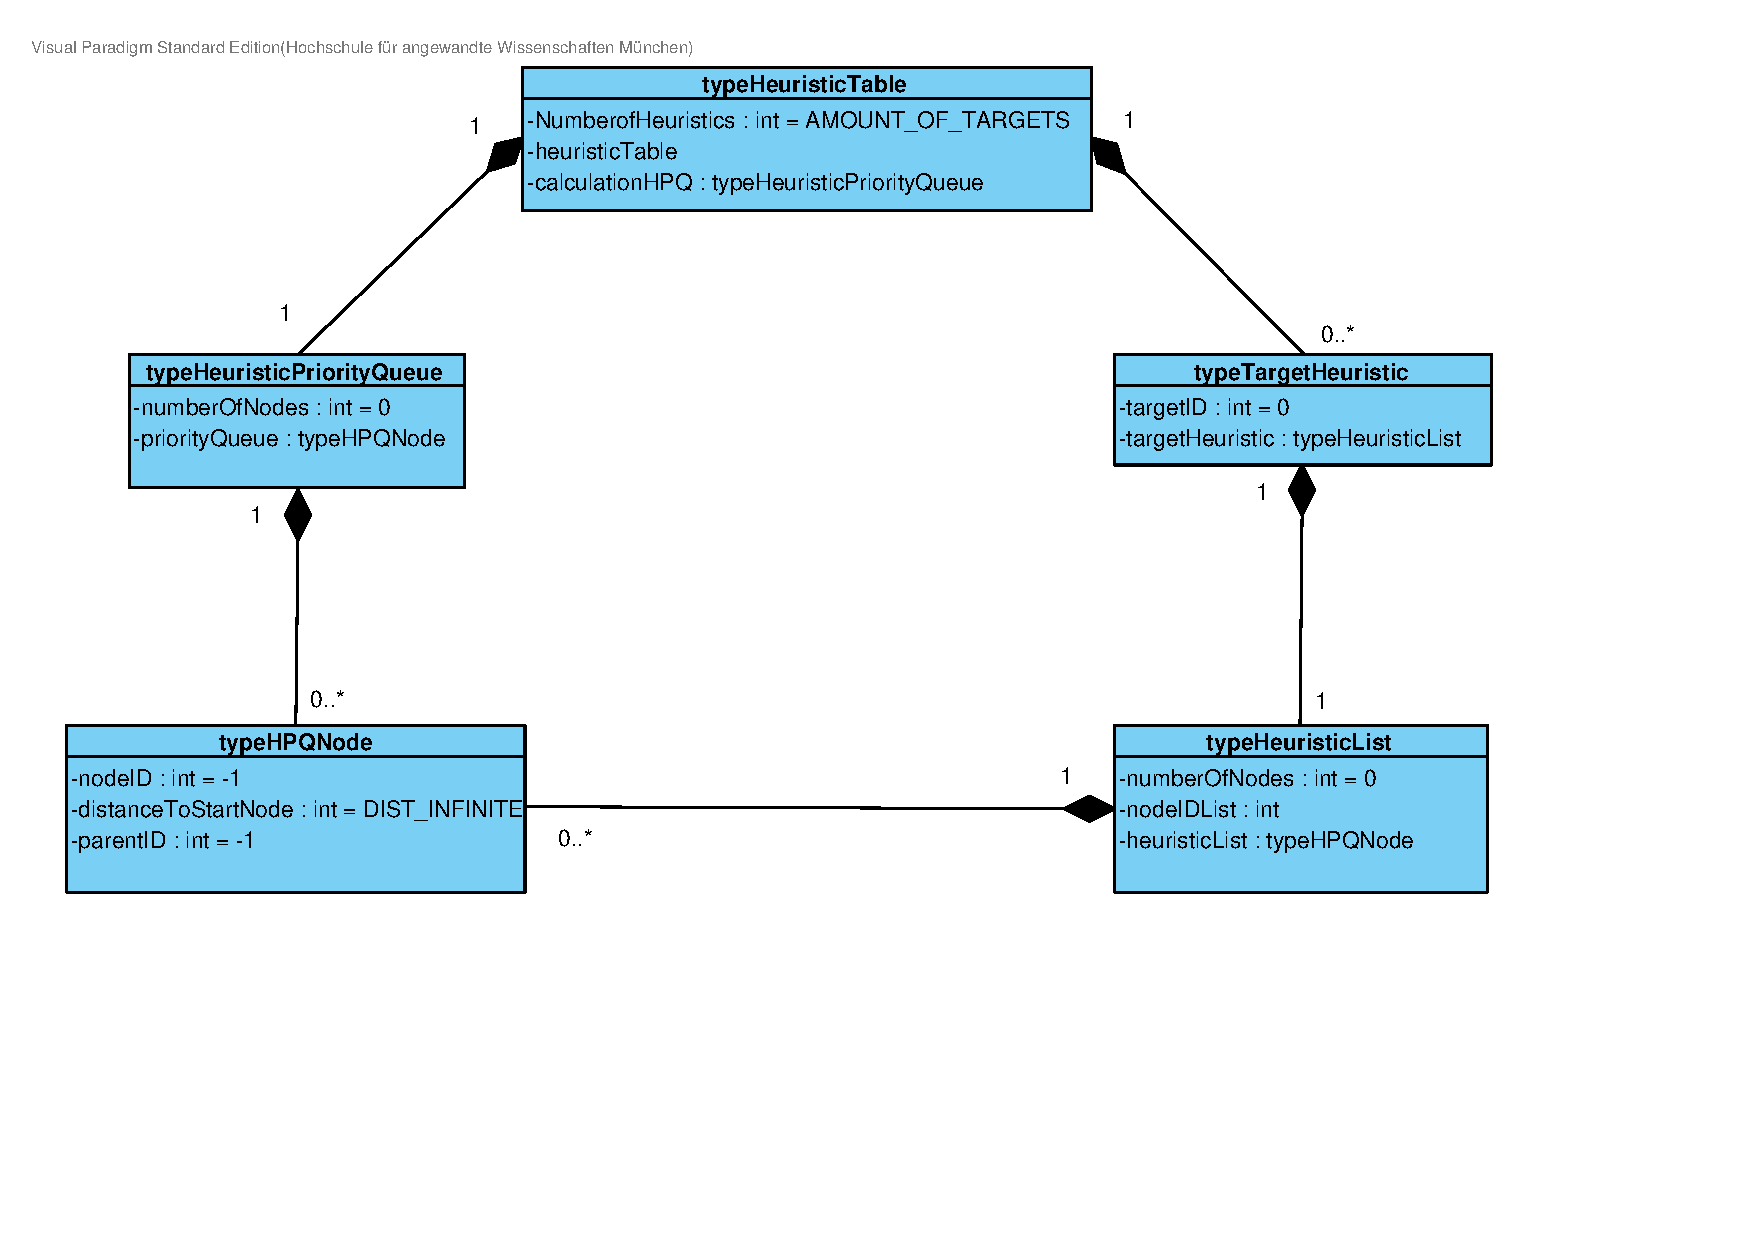
\includegraphics[scale=0.55,trim=0mm 50mm 0mm 0mm ,clip]{/Bilder/HeuristikTabelleUMLPDF}
		\vspace{0.2cm}
		\caption{Aufbau der Datentypen am Beispiel des Datentyps für die Heuristiktabelle.}
	\end{figure}
	 Der Datentyp "`typeHeuristicTable"' besteht aus der zur Berechnung benötigten Priority-Queue und aus einem Feld von Heuristiklisten, welche jeweils einem bestimmten Zielknoten zugeordnet sind.
	
\section{Video der Anlage mit 3 Fahrzeugen}
	Dieser Arbeit liegt ein Video der Funktionsweise der Anlage mit 3 Fahrzeugen bei.
	
	\clearpage
	\phantomsection
	\addcontentsline{toc}{section}{Literaturverzeichnis}
	\bibliographystyle{ieeetr}
	\bibliography{Sources}
		
	\clearpage
	\phantomsection
	\addcontentsline{toc}{section}{\listfigurename}
	\listoffigures
	
	\clearpage
	\phantomsection
	\addcontentsline{toc}{section}{\listtablename}
	\listoftables
	